
\section{Einleitung}
In diesem Versuch wird die Ablenkung eines Elektronenstrahls in einem magnetischen und
einem elektrischen Feld untersucht. Dabei wird die spezifische Ladung der Elektronen,
und die Intensität des Erdmagnetfeldes bestimmt.
\section{Theorie}
\subsection{Aufbau einer Kathodenstrahlröhre}
Um die Ablenkungen des Elektronenstrahls messen zu können, muss eine Kathodenstrahlröhre
verwendet werden. Innerhalb dieses Vakuums kann es nicht zur Wechselwirkung zwischen
Elektronen und Luftmolekülen kommen. Die Kathodenstrahlröhre besteht aus einer
„Elektronenkanode", indem die freien Elektronen erzeugt werden, einem Ablenk- und einem
Nachweissystem.
\newline
Die freien Elektronen werden durch eine Glühemission erzeugt.
Dabei wird die Kathode durch einen Strom erhitzt.
Die Kathode ist von einem Wehnelt-Zylinder umgeben.
Sein negatives Potential macht es möglich die Intensität des Elektronenstrahl zu
steuern.
\newline
Der Aufbau der Kanodenstrahlröhre ist in Abbildung \ref{fig:aufbau} zu sehen.
\begin{figure}
 \centering
  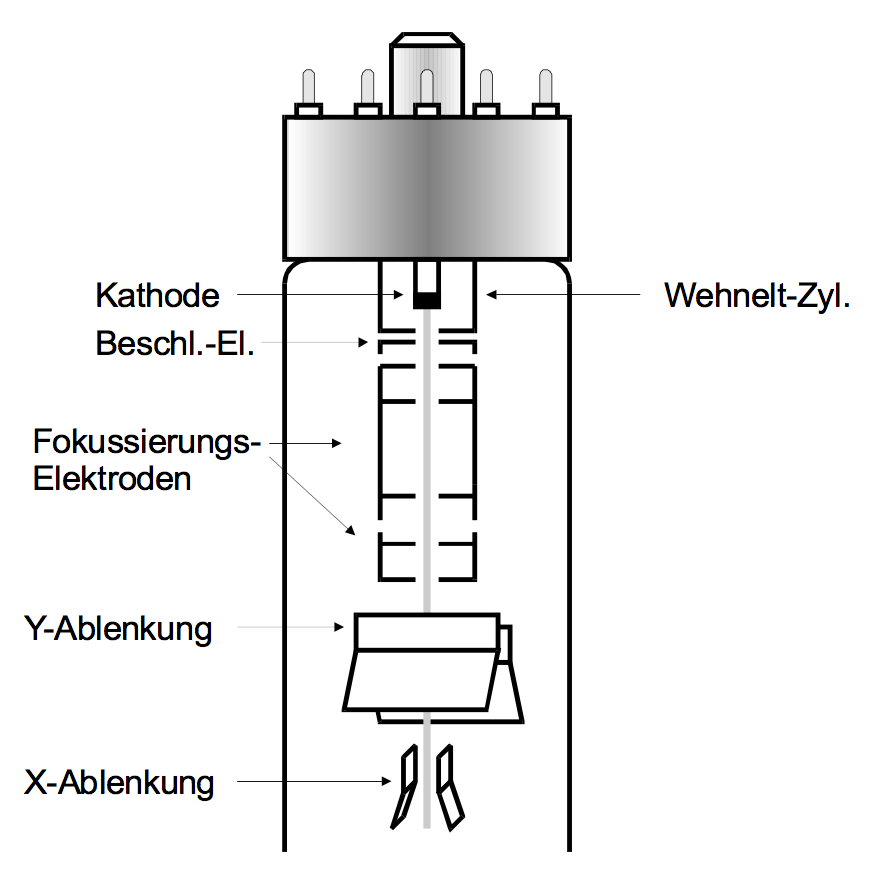
\includegraphics[scale=0.5]{aufbau.png}
  \caption{Querschnitt einer Kathodenstrahlröhre\cite{Anleitung}}
  \label{fig:aufbau}
\end{figure}
\newpage
\subsection{Ablenkung im elektrischen Feld}
In einem homogenen elektrischen Feld ist auf ein Elektron wirkende Kraft $\vec{F}$ durch
\begin{equation}
  \label{eqn:kraft}
  |\vec{F}| = |e_0\vec{E}| = e_0\frac{U_d}{d}
\end{equation}
gegeben. Die Geschwindigkeit $v_y$ der in y-Richtung gleichmäßig beschleunigte Bewegung kann durch
\begin{equation}
  v_{y} = \frac{F}{m_0}{\Delta t}
  \label{eqn:vy}
\end{equation}
beschrieben werden. Aus Gleichung \ref{eqn:kraft} und \ref{eqn:vy} folgt dann
\begin{equation}
	v_{y} = \frac{e_0\cdot U_d\cdot\Delta t}{m_0\cdot d}.
\end{equation}
Die Verschiebung des Leuchtflecks D wird durch
\begin{equation}
	D = \frac{e_0\cdot L\cdot U_d\cdot p}{m_0 \cdot d\cdot v^2}
  \label{eqn:dud}
\end{equation}
beschrieben.
\newline
\begin{figure}
 \centering
  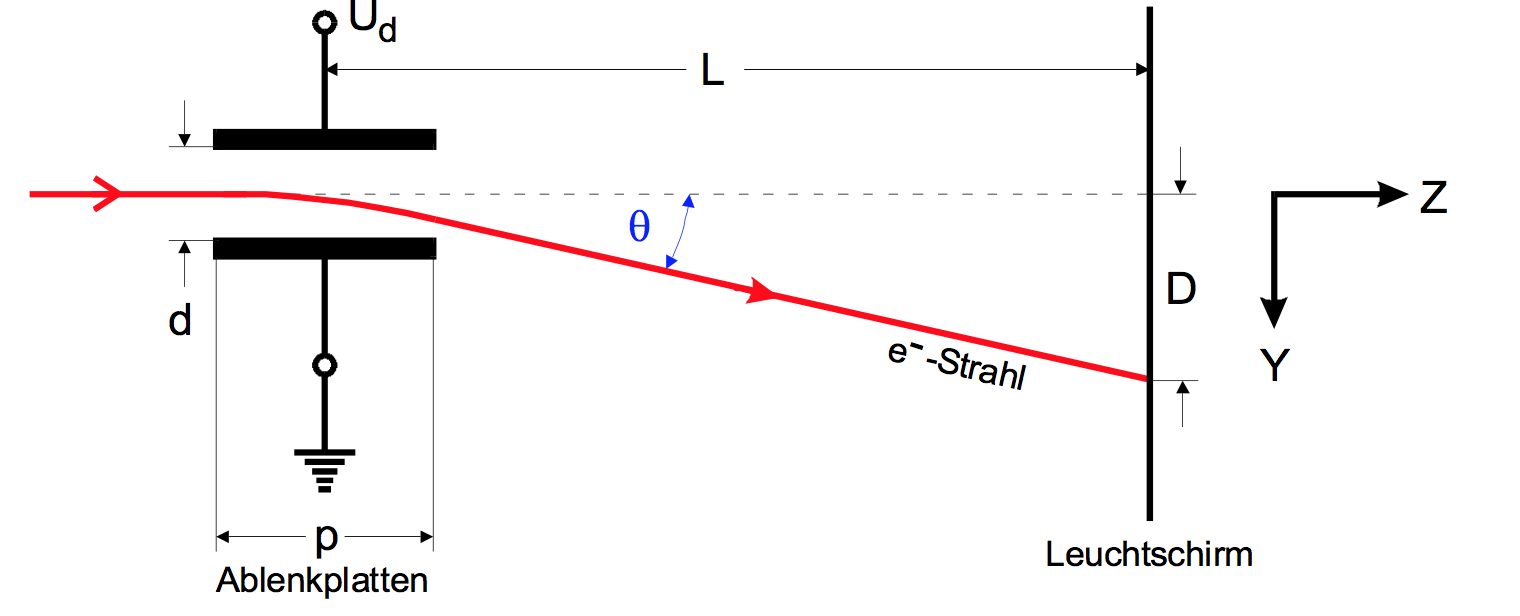
\includegraphics[scale=0.5]{ablenkunge.png}
  \caption{Strahlablenkung in einer Kathodenstrahlröhre\cite{Anleitung}}
  \label{fig:aufbaue}
\end{figure}
\newpage
\subsection{Prinzip des Kathodenstrahl-Oszillographen}
Mit einem Kathodenstrahl-Oszillographen wird die Zeitabhängigkeit von Wechselspannungen
dargestellt. Hierfür wird eine Sägezahnspannung an ein in x-Richtung ablenkendes
Plattenpaar angelegt. An die in y-Richtung ablenkenden Platten wird die zu untersuchende
Spannung angeschlossen. Die Synchronisationsbedingung ist erfüllt, wenn Sägezahn- und Wechselspannungsfrequenz
in einem geeigneten Verhältnis zueinander stehen. Für
\begin{equation}
n \cdot \nu_\text{sä} = m\cdot \nu_\text{we}
\end{equation}
\newline
mit n, m $\in$ N ist dies der Fall.
\subsection{Ablenkung im magnetischen Feld}
Bewegt sich ein geladenes Teilchen mit Geschwindigkeit $\vec{v}$ und Ladung q im magnetischen Feld $\vec{B}$, wirkt auf dieses die Lorentzkraft
\begin{equation}
  \vec{F} = q (\vec{v} \times \vec{B}).
\end{equation}
Durch das Gleichsetzen von Lorentz- und Zentripetalkraft gilt für den Krümmungsradius
\begin{equation}
  r = \frac{m_0v_0}{e_0B}.
\end{equation}
Die Verschiebung des Leuchtflecks D auf dem Leuchtschirm ist durch
\begin{equation}
  r = \frac{L^2 + D^2}{2D}
\end{equation}
gegeben. Die spezifische Ladung der Elektronen $\frac{e_0}{m_0}$ kann dann durch
\begin{equation}
  \frac{L^2 + D^2}{2D} = \frac{m_0v_0}{e_0B}
  \label{eqn:ladung}
\end{equation}
bestimmt werden.
\newline
Durch das Einschalten der Helmholtzspule ergibt sich für die Flussdichte B im Mittelpunkt
\begin{equation}
 B = \mu_0\frac{8NI}{\sqrt{125}R}
 \label{eqn:hh}
\end{equation}
\newline
mit der magnetischen Feldkonstanten $\mu_0$= 4$\pi$$\cdot\num{e-7}$\,$\frac{N}{A^2}$.
\begin{figure}
 \centering
  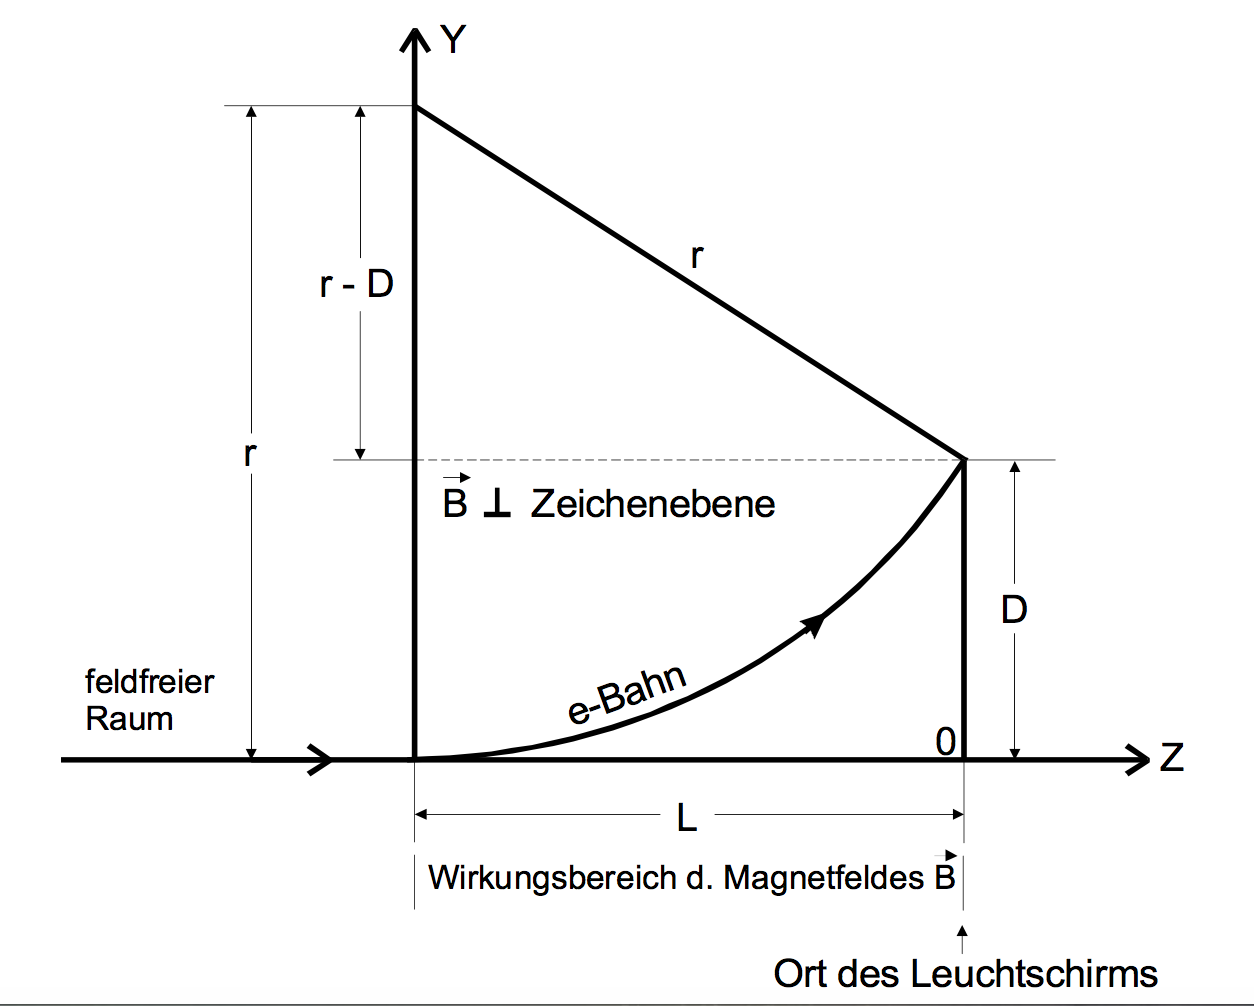
\includegraphics[scale=0.4]{ablenkungm.png}
  \caption{Skizze zur Ableitung einer Beziehung zwischen L, D und r.\cite{Anleitung}}
  \label{fig:aufbaum}
\end{figure}
\newpage
\section{Durchführung}
Zu Beginn des Versuchs wird je eine Platte der X- und Y-Achsensysteme geerdet.
Danach wird die Messapparatur eine Minute lang erhitzt. Erst danach kann eine
Hochspannung angelegt werden. Die Spannung wird so eingestellt, dass der Leuchtfleck
so klein und scharf wie möglich ist. Dieser wird zu erst auf das unterste Gitter des Schirm
zentriert.
\subsection{Bestimmung der spezifischen Ladung der Elektronen}
Unter fünf unterschiedlichen Beschleunigungsspannungen $\su{U_B}$ zwischen 230 und 450\,V wird die Auslenkung in Abhängigkeit
des Stroms gemessen. Dafür wird der Leuchtfleck auf die unterste Vertikale gelegt. Von da aus wird an jeder
Vertikale der Strom $\su{I_d}$ aufgenommen.
\subsection{Bestimmung der Intensität des lokalen Erdmagnetfeldes}
Zur Bestimmung der Intesität des Erdmagnetfeldes wird die Kanodenstrahlröhre in Nord-Süd-
Richtung ausgerichtet und die Helmholtzspule ausgeschaltet. Der Leuchtfleck wird in den Koordinatenursprung gelegt.
Anschließend wird die Apparatur in Ost-West-Richtung gedreht, die Helmholtzspule wieder eingeschaltet
und die Ablenkung des Leuchtflecks durch einen Spulenstrom kompensiert. Durch das Einschalten der Helmholtzspule
wird ein magnetisches Feld erzeugt. Das Spulenfeld gleicht dann genau das horizontale Magnetfeld der
Erde aus.
\newline
Für die Bestimmung der Totalintensität muss Inklinationswinkel $\varphi$ gemessen werden. Der Inklinationswinkel
ist der Winkel zwischen Horizontalebene und der Richtung des Erdmagnetfeldes. Um diesen Winkel zu bestimmen, wird ein Inklinatorium verwendet.
Das Inklinatorium wird in Nord-Süd-Richtung eingestellt, sodass der Flächennormalenvektor senkrecht zum Boden steht.
Danach wird das Inklinatorium um $90\si{\degree}$ gedreht. Jetzt steht der Flächennormalenvektor
parallel zum Boden und der Inklinationswinkel kann abgelesen werden.
\subsection{Proportionalitätsüberprüfung}
Für dieselben Beschleunigungspannungen $\su{U_B}$ zwischen 230 und 450\,V wird die Proportionalität zwischen Ablenkspannung
und Leuchtfleckverschiebung untersucht. Dabei wird wieder der Leuchtfleck zuerst auf die unterste Vertikale gelegt
und danach auf jede andere Vertikale. Im Gegensatz zum ersten Versuchsteil wird hier allerdings die Spannung $\symup{U_d}$
in Abhängigkeit der Auslenkung D gemessen.
\subsection{Kathodenstrahl-Oszillograph}
Im letzten Versuchsteil werden stehende Wellen einer Sinusspannungen erzeugt. Bei einer konstanten Beschleungigunsspannung von 400\,V
werden die Frequenz und die Auslenkung für die vier Fälle n= $\frac{1}{2}$, 1, 2, 3
\begin{equation}
n \cdot \nu_\text{sä} = \nu_\text{si}
\end{equation}
aufgenommen.
